\documentclass[a4paper]{llncs}
\usepackage[T1]{fontenc}
\usepackage[utf8]{inputenc}
\usepackage{lmodern}
\usepackage[scaled=.8]{beramono}
\usepackage{latexsym}
\usepackage{textcomp}

\usepackage{listings}
\lstset{numbers=left, captionpos=b, frame=single, basicstyle=\ttfamily, stringstyle=\small, breaklines=true, extendedchars=true, showstringspaces=true, numberbychapter=false}

\usepackage{graphicx}
\usepackage{multirow}
\usepackage{booktabs}
\usepackage{tabularx}
\usepackage{ctable}
\usepackage{array}
\usepackage{hyperref}
\usepackage{enumitem}
\setlist[itemize,enumerate]{leftmargin=*}

\def\sectionautorefname{Section}
%\renewcommand{\bibname}{References}

\begin{document}



\title{Linked Data Notifications: a resource-centric communication protocol}

\author{Sarven Capadisli\inst{1}
  \and Amy Guy\inst{2}
  \and Christoph Lange\inst{1,3}
  \and Sören Auer\inst{1,3}
  \and Andrei Sambra\inst{4}
  \and Tim Berners-Lee\inst{4}}
\institute{%
  University of Bonn, Bonn, DE
  \email{info@csarven.ca, \{langec,auer\}@cs.uni-bonn.de}
  \and School of Informatics, University of Edinburgh, Edinburgh, UK
  \email{amy@rhiaro.co.uk}
  \and Fraunhofer IAIS, Sankt Augustin, DE
  \and Decentralized Information Group, CSAIL, MIT, Cambridge, US
  \email{deiu@mit.edu, timbl@w3.org}
}
\maketitle

\begin{abstract}
  In this article we describe the Linked Data Notifications (LDN) protocol, which is a W3C Candidate Recommendation. Notifications are sent over the Web for a variety of purposes, for example, by social applications. The information contained within a notification is structured arbitrarily, and typically only usable by the application which generated it in the first place. In the spirit of Linked Data, we propose that notifications should be reusable by multiple authorised applications. Through separating the concepts of {\em senders}, {\em receivers} and {\em consumers} of notifications, and leveraging Linked Data principles of shared vocabularies and URIs, LDN provides a building block for decentralised Web applications. This permits end users more freedom to switch between the online tools they use, as well as generating greater value when notifications from different sources can be used in combination. We situate LDN alongside related initiatives, and discuss additional considerations such as security and abuse prevention measures. We evaluate the protocol’s effectiveness by analysing multiple, independent implementations, which pass a suite of formal tests and can be demonstrated interoperating with each other. To experience the described features please open this document in your Web browser under its canonical URI: {\tt \href{http://csarven.ca/linked-data-notifications}{http://csarven.ca/linked-data-notifications}}.
  \keywords{Communications protocol, Decentralisation, Linked Data, Social web}
\end{abstract}

                        \section{Introduction}
  \label{introduction}



\par Notifications are sent over the Web for a variety of purposes, including social applications: ``You have been invited to a graduation party!'', ``Tim commented on your blog post!'', ``Liz tagged you in a photo''. The notification data may be displayed to a human to acknowledge, or used to trigger some other application-specific process (or both). In a decentralised architecture, notifications can be a key element for federation of information, and application integration. However in centralised systems which prevail today, this data is structured arbitrarily and typically only usable by the application that generated it in the first place. Current efforts towards {\em re-decentralising} the Web~\cite{ref-1,ref-2,ref-3} are moving towards architectures in which data storage is decoupled from application logic, freeing end users to switch between applications, or to let multiple applications operate over the same data. So far, notifications are considered to be {\em ephemeral} resources which may disappear after transport, and thus are excluded from being designed for reuse.


\par We argue that notification data should not be locked into particular systems. We designed the {\em Linked Data Notifications (LDN)} protocol to support sharing and reuse of notifications {\em across} applications, regardless of how they were generated or what their contents are. We describe how the principles of identification, addressability and semantic representation can be applied to notifications on the Web. Specifying LDN as a formal protocol allows independently implemented, heterogeneous applications which generate and use notifications, to seamlessly work together. Thus, LDN supports the decentralisation of the Web as well as encourages the generation and consumption of Linked Data.


\par We build on existing W3C standards and Linked Data principles. In particular, the storage of notifications is compatible with the Linked Data Platform standard; notifications are identified by HTTP URIs; and notification contents are available as JSON-LD. A key architectural decision is the separation of concerns between {\em senders}, {\em receivers}, and {\em consumers} of notifications. Implementations of the protocol can play one or more of these roles, and interoperate successfully with implementations playing the complementary roles. This means that notifications generated by one application can be reused by a completely different application, accessed via the store where the notification data resides, through shared Linked Data vocabularies. LDN also pushes the decentralised approach further by allowing any {\em target} resource to advertise its Inbox anywhere on the Web; that is, targets do not need to be coupled to or controlled by a receiver, and can make use of a third-party {\em Inbox as a service}.


\par LDN is a W3C \empty Candidate Recommendation via the \empty Social Web Working Group~\cite{ref-4}. The first two authors of this article co-edited the specification.


\par Use cases for decentralised notifications are particularly evident in social networking (status updates, interactions, games); scholarly communication (reviews, citations); and changes of state of resources (datasets, versioning, sensor readings, experimental observations). We describe the requirements which guided the development of the protocol and discuss related work, including current alternative approaches and complementary protocols which can work alongside LDN. We summarise the protocol itself, and specific architectural considerations that were made. We built a test suite which can be used to confirm that implementations conform with the specification, and we describe 17 implementations which interoperate with each other.



\par As the following terms used throughout this article may be subject to different interpretations by different communities, we provide some definitions here.


\par By decentralisation, we mean data and applications are loosely coupled, and users are empowered to choose where their data is stored or held. We focus on Web-based decentralisation, where content is transported over HTTP, and resources are identified with URIs. An Inbox is a container or directory (attached to a Web resource) which is used to store and serve a collection of notifications. A notification is a retrievable resource which returns RDF. The contents of notifications are intended to describe a change in state of some other resource, or contain new information for the attention of a user or process, and may be subject to constraints of the Inbox it is contained in.








                        \section{Related Work}
  \label{related-work}



\par Here we review previous and ongoing efforts towards delivering notifications in a decentralised manner. Many systems which make use of notifications operate either in a completely centralised way, or are decentralised only in the sense that different instances of the {\em same} codebase need to interoperate; we restrict our review to mechanisms which do not expect the notification to be received or used only by the same software or platform which sent it.


\par The contents of a notification is either: 1) URLs, indicating relations between Web resources, or 2) a ‘fat ping’ containing a blob of information. Semantic Pingback, Webmention, and Provenance Pingback follow the first form, and are also known as linkbacks, the suite of protocols that essentially allows Web documents to automatically reciprocate hyperlinks. This has the advantage that a verification mechanism can be tightly specified (the URL of the target must appear in the content of the source), but the disadvantage that notifications are only available for use cases involving Web publishing.


\par \empty Semantic Pingback~\cite{ref-2} and \empty Webmention~\cite{ref-5} both update the original \empty Pingback~\cite{ref-6} mechanism by replacing the XML-RPC transport mechanism by a {\tt x-www-form-urlencoded} request with two parameters ({\tt source} and {\tt target}). Resources which are the target for a notification advertise the respective receiving service or endpoint via a {\tt Link} relation, either in HTTP headers or HTML. Semantic Pingback additionally enables discovery of the Pingback service where target is available as RDF. While the content at source may indicate (in any convention or serialisation format) the type of relation between the source and target URLs, this information about the relation is not transmitted to the receiver’s endpoint; only the source and target URLs are sent. As such, there is also no way to distinguish between multiple potential mentions of the target at the source; this is left up to the receiver to interpret. Semantic Pingback does encourage generation of additional semantics about the relation(s) between the source and the target by processing the source as RDF if possible, and also defines specific ways for a receiving server to handle incoming pingback data in order to add the source data to an RDF knowledge base~\cite{ref-2}. Beyond verifying that the source contains the URL of the target, Webmention does not specify any further requirements of the receiving server; nor is it expected that “mentions” are retrievable once they have been sent.


\par A \empty Provenance Pingback endpoint is also advertised via the HTTP {\tt Link} header; it accepts a list of URIs for provenance records describing uses of the resource~\cite{ref-7}. Provenance Pingback does not specify any further behaviour by the receiving server, but the contents at the URIs listed in the notification body must be semantic data.


\par Other notification mechanisms send more information than just URLs in the notification body; due to each mechanism’s focused use case, the payload is restricted to a particular vocabulary.


\par \empty DSNotify is a centralised service which crawls datasets and observes changes to links with the specific use case of preserving link integrity between Linked Open Data resources. Third-party applications can register with the sending service to receive notifications of changes in the form of a specific XML payload~\cite{ref-8}. With the \empty sparqlPuSH service, users may input a SPARQL query, the results of which are the specific updates they are interested in. The query is run periodically by the service, and the results are converted to RSS and Atom feeds, which is sent to a \empty PubSubHubbub hub to which the user can subscribe~\cite{ref-9}. The \empty ResourceSync Change Notification specification also sends update notifications via a PuSH hub, this time with an XML payload based on the Sitemap format~\cite{ref-10}. Each of these mechanisms is triggered by subscription requests. That is, a user must actively solicit messages from a particular service, rather than having a way for a service to select a notification target and autonomously discover where to send notifications to.




                        \section{Requirements and Design Considerations}
  \label{requirements-and-design-considerations}



\par In this section we discuss our considerations for a Web notification protocol that conforms to the Linked Data design principles, as well as best practices for applications. We use these considerations to establish both concrete requirements and points of implementation-specific flexibility for the protocol.


                                \subsection{R1 Modularity}
  \label{modularity}



\par To encourage modularity of applications, one should differentiate between different classes of implementation of the protocol. Two parties are involved in the creation of a notification: a {\em sender}, generating the notification data, and a {\em receiver}, storing the created resource. We also have the role of a {\em consumer}, which reads the notification data and repurposes it in some way. A software implementation can of course play two or all three of these roles; the important part is that it need not. A consuming application can read and use notification data without being concerned about ever sending or storing notifications.




                                \subsection{R2 Reusable notifications}
  \label{reusable-notifications}



\par The relationship between the {\em consumer} and {\em receiver} roles is key to notifications being reusable. A consumer must be able to autonomously find the location of notifications for or about the particular resource it is interested in. To achieve this we place a requirement on the receiver to expose notifications it has been sent in such away to permit other applications to access them; and specify how any resource can advertise its receiving endpoint for consumers to discover. To promote fair use or remixing of notification contents, applications can incorporate rights and licensing information into the data. Similarly, applications may include additional information on licensing resources that the notification refers to. The presence of this type of information is important for consumers to assess the (re)usability of data.




                                \subsection{R3 Persistence and Retrievability}
  \label{persistence-and-retrievability}





\par There is a social expectation and technical arguments for ensuring the persistence of identifiers of Web resources~\cite{ref-11}. This is inconsistent with the traditionally ephemeral nature of notifications. Applications may benefit from referring to or reusing notifications if the notifications are known to be available in the long term, or indicate their expected lifespan~\cite{ref-12}.


\par A {\em RESTful architecture}~\cite{ref-13} is well suited for persistent notifications, as it involves organisation of atomic resources, their discovery and description, and a lightweight API for the CRUD (create, read, update, and delete) operations~\cite{ref-14}. This enforces the notion that notifications are considered resources in their own right, with their own dereferencable URIs.


\par We need to consider both the needs of software systems and humans when large amounts of notification data are being generated and shared between diverse applications which may be operating without knowledge of each other. To organise and manage large amount of notifications over time, mechanisms should be in place to break representations of collections of notifications into multiple paged responses that may be easier to consume by applications.


\par Relatedly, receivers may carry out resource management or garbage collection, or permit consumers or other applications to do so. For example, an application to consume messages might let an authenticated and authorised user ‘mark as read’ by adding a triple to the notification contents.




                                \subsection{R4 Adaptability}
  \label{adaptability}





\par Linked Data applications benefit from domain-driven designs; that is, functionality being small and focussed on a particular purpose, rather than generic. We believe a notification protocol should be adaptable for different domains, but that there is no need to create multiple domain-specific notification protocols; the fundamental mechanics are the same.


\par R4-A: Any resource may be the {\em target} of a notification. By target, we mean a notification may be addressed {\em to} the resource, be {\em about} the resource, or for a sender to otherwise decide that it is appropriate to draw the attention of the resource (or resource owner) to the information in the notification body. As such, any Web resource must be able to advertise an endpoint to which it can receive notifications. Resources can be RDF or non-RDF (such as an image, or CSV dataset), and may be informational (a blog post, a user profile) or non-informational (a person).


\par R4-B: We do not purport to be able to design a notifications ontology which is appropriate for every domain. Thus we consider the {\em contents} of a notification to be application specific. From a sender’s perspective, we derive two core principles: a notification can contain {\em any data}; a notification can use {\em any vocabulary}. From a consumer’s perspective, interoperability between different applications occurs through vocabulary reuse, and shared understanding of terms. This is in accordance with Linked Data principles in general. The practical upshot of this is that a calendar application which consumes event invitations using the \empty RDF Calendar vocabulary is likely to completely ignore notifications containing the \empty PROV Ontology, even if it finds them all stored in the same place. For two independent applications operating in the {\em same} domain, a shared understanding of appropriate vocabulary terms is assumed.



\par However from a receiver’s perspective, exposing itself to receive any blobs of RDF data from unknown senders may be problematic. Thus, R4-C: it should be possible for the receiver to enforce restrictions and accept only notifications that are acceptable according to its own criteria (deemed by e.g., user configuration; domain-specific receivers). This can be used as an anti-spam measure, a security protection, or for attaining application and data integrity.


\par Rejecting notifications which do not match a specific pattern in their contents, or the {\em shape} of the data, is one way to filter. For example, if the Inbox owner knows that they will only ever use a consuming application which processes friend requests, they can configure their receiver to filter out anything that does not match the pattern for a friend request, helping their consumer to be more efficient. If the notification constraints are also advertised by the receiving service as structured descriptions, generation and consumption of the notifications can be further automated. Possible specifications for doing so are W3C \empty Shapes Constraint Language (SHACL)~\cite{ref-15} or \empty ShEx.


\par Receivers may wish to filter notifications by verifying the sender, through for example a whitelist or a Web of trust. This requires an authentication mechanism and since different authentication mechanisms are appropriate for different applications, the notification protocol should ideally be usable alongside various methods such as clientside certificates, e.g., WebID+TLS, token-based, e.g., OAuth 2.0, or digital signatures.


\par As ``anyone can say anything about anything'' a receiver may choose to resolve any external resources referred to by the notification, and cross-check the notification contents against authoritative sources. This is similar to how Semantic Pingback and Webmention require fetching and parsing of the source URL to verify existence of the target link.





                                \subsection{R5 Subscribing}
  \label{subscribing}



\par In general, applications may require that new notifications are pushed to them in real-time, or to request them at appropriate intervals. To take this into account, we expand our definition of senders, receivers and consumers with the following interaction expectations: notifications are {\em pushed} from senders to receivers; and {\em pulled} from receivers by consumers.


\par Thus, an application which offers an endpoint or callback URL to which notifications should be sent directly is a receiver, and an application which fetches notifications from an endpoint on its own schedule is a consumer. Much of the related work {\em requires} notifications to be explicitly solicited to trigger sending. Since in a decentralised model, receivers may not be aware of possible sources for notifications, our sender-receiver relationship depends on the sender’s autonomy to make such decisions by itself. This does not preclude the scenario in which a receiver may wish to solicit notifications from a particular sender, but as there are already subscription mechanisms in wide use on the Web, we do not need to specify it as part of LDN. For example, \empty WebSub (recent W3C evolution of PubSubHubbub), the WebSocket Protocol, or HTTP Web Push.




\par Given our adoption of Linked Data principles and a RESTful architecture, a further design decision was to ensure minimal compatibility with the \empty Linked Data Platform (LDP) specification~\cite{ref-16}. LDP is a RESTful read-write API for RDF resources, which groups related resources together into constructs known as ``Containers''. Thus, existing LDP servers can be used to store notifications, as new notifications can be created by {\tt POST}ing RDF to a container.




                        \section{The LDN Protocol}
  \label{protocol}



\par The {\em Linked Data Notifications (LDN)} protocol describes how servers (receivers) can receive messages pushed to them by applications (senders), as well as how other applications (consumers) may retrieve those messages. Any resource can advertise a receiving endpoint (Inbox) for notification messages. Messages are expressed in RDF, and can contain arbitrary data. It is not dependent on a complete implementation of LDP, but comprises an easy-to-implement subset.


\begin{figure}
  \centering
  \includegraphics[trim=.2cm 10cm .5cm 10cm,clip,width=.6\textwidth]{media/images/{linked-data-notifications-overview.svg}.pdf}
  \caption{Overview of Linked Data Notifications}
  \label{fig:overview}
\end{figure}


                                \subsection{Sender to receiver interactions}
  \label{sender-to-receiver}



\par The following steps (in order without skipping) describe the interaction between sender and receiver:


\par (1) A sender is triggered, either by a human or an automatic process, to deliver a notification; (2) The sender chooses a target resource to send notifications to; (3) The sender discovers the location of the target’s {\em Inbox} through the {\tt ldp:inbox} relation in the HTTP {\tt Link} header or RDF body of the target resource; (4) The sender creates the body of the notification according to the needs of application; (5) The sender makes a {\tt POST} to the Inbox URL, containing the body in JSON-LD or in another serialisation acceptable by the server; (6) The receiver optionally applies filtering rules, and sends the appropriate HTTP response code to accept or reject the notification; (7) The receiver exposes the notification data (according to appropriate access control) for use by consumers.




                                \subsection{Consumer to receiver interactions}
  \label{consumer-to-receiver}



\par The following steps (in order without skipping) describe the interaction between consumer and receiver:


\par (1) A consumer selects a target and discovers the location of its Inbox in the same way as the sender; (2) A receiver responds to {\tt GET} requests made to the Inbox URL with a listing of the URLs of notifications that have previously been accepted, linked to the Inbox with the {\tt ldp:contains} predicate; (3) The receiver responds to {\tt GET} requests made to the individual notification URLs with JSON-LD (or optionally other serialisations); (4) Following the retrieval of notification listings or individual notifications, the consumer may perform further processing, combine with some other data, or simply present the results in a suitable human-readable way.




                                \subsection{Example Notifications}
  \label{example-notifications}



\par For more example notification payloads, see the \empty LDN specification.


\begin{lstlisting}
{ "@context": { "sioc": "http://rdfs.org/sioc/ns#" }
  "@id": "",
  "@type": "sioc:Comment",
  "sioc:content": "This is a great article!",
  "sioc:reply_of": { "@id": "http://example.org/article" },
  "sioc:created_at": { "@value": "2015-12-23T16:44:21Z" } }
\end{lstlisting}
                                        A notification about a comment created by a user (JSON-LD).



\begin{lstlisting}
@prefix as: <https://www.w3.org/ns/activitystreams#> .
@prefix cito: <http://purl.org/spar/cito/> .
<> a as:Announce
  as:object <https://linkedresearch.org/resources#r-903b83> ;
  as:target <http://csarven.ca/dokieli#architecture> .
<https://linkedresearch.org/resources#r-903b83>
  cito:citesAsPotentialReading
    <http://csarven.ca/linked-data-notifications#protocol> .
\end{lstlisting}
                                        An announcement of a specific citation relation between two entities (Turtle).







                        \section{Implementations}
  \label{implementations}



\par Here we summarise the 17 LDN implementations we are aware of to date. They are built by 10 different teams or individuals using different tool stacks (5 clientside JavaScript, 3 PHP, 3 NodeJS, 3 Python, 1 Perl, 1 Virtuoso Server Pages, 1 Java) and have submitted \empty implementation reports as part of the W3C standardisation process. We note that any \empty LDP implementation is a conforming LDN receiver; we refer here to the ones we have tested. We discuss the value of these implementations further in the \empty Evaluation section.

\ctable[
  caption={LDN Implementations},
  label = {tab:implementations}
]{lll}{
  \tnote[*]{Conformance classes: S – sender, C – consumer, R – receiver.}
  \tnote[a]{Implementations by the authors}
  \tnote[]{Source: \url{https://github.com/w3c/ldn}}
}{\FL
  Implementation & Class\tmark[*] & Description
  \ML
                                        CarbonLDP &
                                        R &
                                        Data storage platform (LDP) \NN


                                        dokieli\tmark[a] &
                                        S,C &
                                        Clientside editor and annotator \NN


                                        errol\tmark[a] &
                                        S &
                                        Generic message sending client \NN


                                        Fedora Commons &
                                        R &
                                        Open source repository platform (LDP) \NN


                                        IndieAnndroid &
                                        R &
                                        Personal blogging platform \NN


                                        Linked Edit Rules &
                                        S &
                                        Statistical dataset consistency checker \NN


                                        mayktso\tmark[a] &
                                        R &
                                        Personal data store (LDP) \NN


                                        OnScreen\tmark[a] &
                                        C &
                                        Notifications display client \NN


                                        pyldn &
                                        R &
                                        Standalone Inbox \NN


                                        RDF-LinkedData-Notifications &
                                        R &
                                        Standalone Inbox \NN


                                        sloph\tmark[a] &
                                        S,R &
                                        Social publishing \& quantified self \NN


                                        Solid Words &
                                        S &
                                        Foreign language learning app \NN


                                        solid-client &
                                        S &
                                        Clientside library for LDP \NN


                                        solid-inbox &
                                        C &
                                        Clientside social message reader \NN


                                        solid-notifications &
                                        S,C &
                                        Clientside library for LDN \NN


                                        solid-server &
                                        R &
                                        Personal data storage server (LDP) \NN


                                        Virtuoso+ ODS Briefcase &
                                        R,C &
                                        Personal data storage server (LDP) \LL
}





\par We highlight social scholarly communication use cases with \empty dokieli, a clientside editor for decentralised scientific article publishing, annotations and social interactions~\cite{ref-17}. dokieli uses LDN to send and consume notifications: When a reader comments on a fragment of text in an article, the application discovers the article’s Inbox and sends a notification about the annotation. dokieli also consumes notifications from this Inbox to fetch and display the annotation as marginalia (figure~\ref{fig:video-annotation}). A reader can share a dokieli-enabled article with their contacts; dokieli discovers each contact’s Inbox and sends a notification there (figure~\ref{fig:video-share}). When editing an article, the author can add a citation. If an Inbox is discovered in the cited article, dokieli sends a notification there to indicate what part of the article was cited by whom and where. dokieli-enabled articles also consume citation notifications to display these metrics for the author and other readers (figure~\ref{fig:like}).

\begin{figure}
  \begin{minipage}[b]{.49\textwidth}
    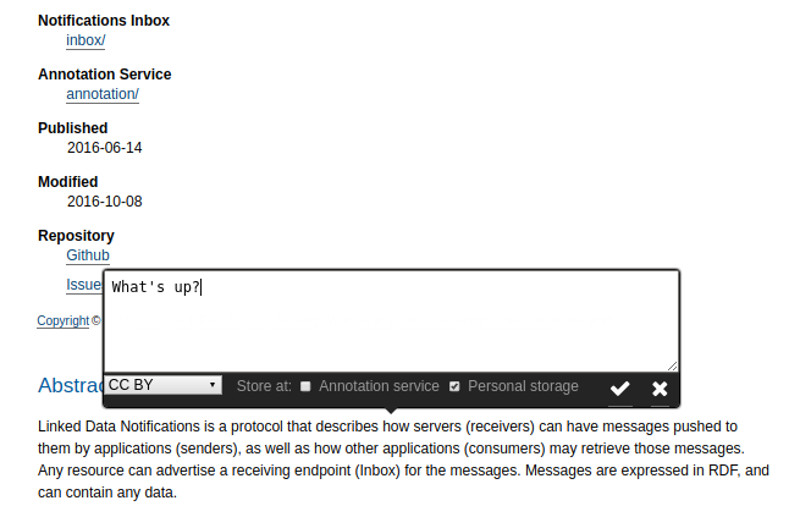
\includegraphics[width=\textwidth]{media/images/dokieli-annotation}
    \caption{Video of dokieli Web Annotation}
    \label{fig:video-annotation}
  \end{minipage}
  \hfill
  \begin{minipage}[b]{.49\textwidth}
    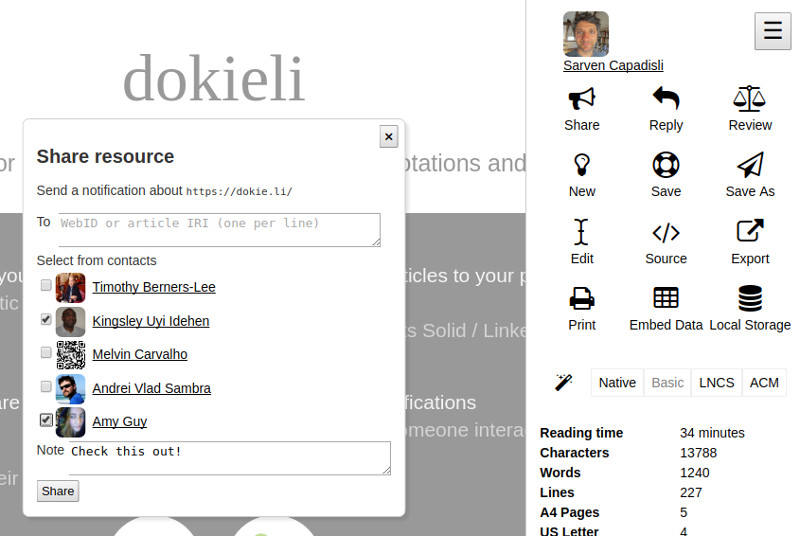
\includegraphics[width=\textwidth]{media/images/dokieli-share}
    \caption{Video of dokieli Share}
    \label{fig:video-share}
  \end{minipage}
\end{figure}






\par Notifications sent by dokieli can be reused by any consuming applications that recognise the vocabulary terms; similarly, dokieli can consume notifications sent by different applications.


\par Further social use cases are demonstrated by \empty sloph, a personal publishing and quantified self platform which acts as a node in a decentralised social network. When new content is created on the server, sloph performs discovery on URLs it finds as values of particular properties of the new content, as well as any URLs in the body of the content, and sends notifications accordingly. For instance:

                            \begin{itemize}
  \item If a {\em Like} activity is generated on the server, sloph uses the {\tt object} of the {\em Like} as the target for a notification. Since dokieli uses the same vocabulary for social interactions (\empty ActivityStreams 2.0~\cite{ref-18}), if the target is a dokieli article, this {\em Like} will be displayed (figure~\ref{fig:like}).\item If the user publishes a blog post containing a link, which may be semantically annotated to indicate the reason for linking, sloph sends a notification to any Inbox discovered at that link.\item As a receiver, sloph accepts all incoming notifications, but holds for moderation (i.e. places behind access control) any that it cannot automatically verify refer to third-party content published on another domain. If an article written with dokieli publishes a citation of a blog post which advertises a sloph Inbox, sloph will fetch the article and verify whether the relation matches the contents of the notification before exposing the notification for re-use.
    \end{itemize}



\par \empty Linked Edit Rules and \empty Solid Words are specialised senders. Linked Edit Rules checks the consistency of statistical datasets against structured constraints, and delivers the consistency report as a notification to the user. Solid Words is a clientside game for learning new words in a foreign language; it delivers the player’s score for each round to their Inbox. \empty OnScreen is a (crude) generic consumer; as such, it can display notifications sent by both of the aforementioned senders (figure~\ref{fig:notifications}).

\begin{figure}
  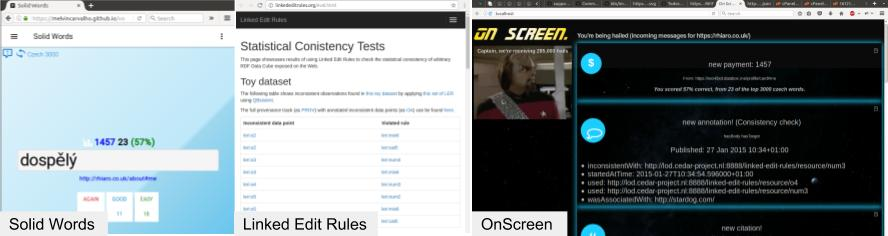
\includegraphics[width=\textwidth]{media/images/screenshot-ldn-sloph-dokieli}
  \caption{A {\em Like} notification created by sloph, displayed by dokieli.}
  \label{fig:like}

  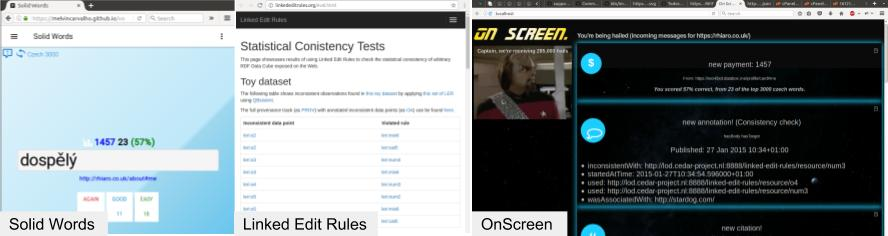
\includegraphics[width=\textwidth]{media/images/screenshot-ldn-senders}
  \caption{A: Solid Words (a sender), B: Linked Edit Rules (a sender), C: OnScreen (a consumer) displaying notifications sent by A and B.}
  \label{fig:notifications}
\end{figure}












                        \section{Analysis and Evaluation}
  \label{analysis-and-evaluation}



\par The LDN protocol describes the discovery of a resource’s Inbox whence notifications are sent or consumed, and the sending and exposure of those notifications. Here we analyse how well features of LDN achieve the \empty requirements identified previously, and compare this to related work.


\par We have already examined \empty implementations of the specification and described how they interoperate with each other; this can be further tested by running the \empty test suite: https://linkedresearch.org/ldn/tests/. We can use this towards an evaluation of its feasibility and effectiveness at interoperability. Given the relatively early stage in the standardisation process (LDN entered Candidate Recommendation in 2016-11), the fast adoption of the LDN specification, quantity of the implementations, and their diversity is promising and further shows LDN’s feasibility. Furthermore, during the development of the specification issues have been raised or discussed by 28 different people (excluding the authors; 21 outside of the Social Web Working Group, 7 within) and the specification has undergone formal review by internationalisation, accessibility, and security specialists. We also discuss in more depth particular challenges that were raised and resolved as part of this process.


                                \subsection{Comparison summary}
  \label{comparison-summary}



\par Here we compare existing notification mechanisms from related work. The criteria includes our \empty requirements and design considerations ({\em Rx}) along with additional technical information which helps to capture some design differences ({\em Tx}).


\begin{table}
  \caption{Comparison of notification mechanisms}
  \label{tab:comparison}
  \footnotesize
  \begin{tabular}{% Mechanism
    p{.14\textwidth}
    % T1–T3
    p{.065\textwidth}
    p{.075\textwidth}
    p{.1\textwidth}
    % R1–R3
    p{.03\textwidth}
    p{.03\textwidth}
    p{.04\textwidth}
    % R4-A–R5
    p{.06\textwidth}
    p{.14\textwidth}
    p{.045\textwidth}
    p{.06\textwidth}
    p{.06\textwidth}
    p{.05\textwidth}
    }\FL
                                                Mechanism&
                                                T1&
                                                T2&
                                                T3&
                                                R1&
                                                R2&
                                                R3&
                                                R4-A&
                                                R4-B&
                                                R4-C\textsuperscript{p}&
                                                R4-C\textsuperscript{v}&
                                                R4-C\textsuperscript{o}&
                                                R5\ML
                                                Semantic\newline Pingback&
                                                Link-\newline back&
                                                POST&
                                                RDF&
                                                S\newline R&
                                                /&
                                                /&
                                                Any\textsuperscript{r}&
                                                form\newline urlencoded\textsuperscript{k}&
                                                !&
                                                !\newline parse\newline source&
                                                Any\textsuperscript{r}&
                                                X\NN
                                                Web-\newline mention&
                                                Link-\newline back&
                                                POST&
                                                HTML&
                                                S\newline R&
                                                –&
                                                –&
                                                Any\textsuperscript{h}&
                                                form\newline urlencoded\textsuperscript{k}&
                                                !&
                                                !\newline parse\newline source&
                                                Any\textsuperscript{h}&
                                                X\NN
                                                Provenance\newline Pingback&
                                                Link-\newline back&
                                                POST&
                                                RDF&
                                                S\newline R&
                                                /&
                                                /&
                                                /&
                                                URI list&
                                                /&
                                                /&
                                                RDF\textsuperscript{q}&
                                                X\NN
                                                DSNotify&
                                                Fat\newline ping&
                                                POST,\newline PUT&
                                                XML,\newline PuSH&
                                                S\newline U&
                                                /&
                                                –&
                                                –&
                                                XML&
                                                /&
                                                –&
                                                RDF\textsuperscript{t}&
                                                !\NN
                                                sparqlPuSH&
                                                Fat\newline ping&
                                                POST&
                                                XML,\newline SPARQL,\newline PuSH&
                                                S\newline U&
                                                –&
                                                –&
                                                –&
                                                XML\textsuperscript{ra}&
                                                /&
                                                –&
                                                RDF\textsuperscript{t}&
                                                !\NN
                                                Resource-\newline Sync&
                                                Fat\newline ping&
                                                POST&
                                                XML,\newline PuSH&
                                                S\newline U&
                                                /&
                                                –&
                                                –&
                                                XML\textsuperscript{s}&
                                                /&
                                                –&
                                                ?&
                                                !\NN
                                                Linked Data\newline Notifications&
                                                Fat\newline ping&
                                                POST&
                                                JSON-LD&
                                                S\newline R\newline C&
                                                !&
                                                !\newline URI&
                                                Any&
                                                JSON-LD\textsuperscript{j}&
                                                + app&
                                                + app&
                                                –&
                                                O\newline app\LL
  \end{tabular}\\
  \begin{tabularx}{1.0\linewidth}{XX}\FL
    \textbf{T1}: Notification type&
    \textbf{R4-A}: Target representation\NN
    \textbf{T2}: Delivery method&
    \textbf{R4-B}: Notification body\NN
    \textbf{T3}: Dependencies&
    \textbf{R4-C\textsuperscript{p}}: Payload processing required?\NN
    \textbf{R1}: Modularity (application classes: S Sender, R Receiver, C Consumer, U Subscriber/User)&
    \textbf{R4-C\textsuperscript{v}}: Verification - required? how?\NN
    \textbf{R2}: Reusability&
    \textbf{R4-C\textsuperscript{o}}: Requirements for referenced resources?\NN
    \textbf{R3}: Persistence - required? how?&
    \textbf{R5}: Subscription\ML
    \textbf{–}: not applicable, out of scope&
    \textbf{!}: required ({\em MUST})\NN
    \textbf{/}: not specified, in scope&
    \textbf{+}: recommended ({\em SHOULD})\NN
    \textbf{X}: explicitly disallowed&
    \textbf{O}: optional ({\em MAY})\NN
    \textbf{app}: application specific decision&
    \textbf{PuSH}: PubSubHubbub\ML
    \textbf{\textsuperscript{h}}: HTML recommended&
    \textbf{\textsuperscript{r}}: RDF representation recommended\NN
    \textbf{\textsuperscript{j}}: Alternate RDF formats can be negotiated&
    \textbf{\textsuperscript{ra}}: SPARQL results transformed to RSS/Atom\NN
    \textbf{\textsuperscript{k}}: {\tt source} and {\tt target} key–value pairs is required&
    \textbf{\textsuperscript{s}}: \empty Sitemaps\NN
    \textbf{\textsuperscript{q}}: Provenance records with \empty PROV Ontology&
    \textbf{\textsuperscript{t}}: Described in an RDF store or dataset\LL
  \end{tabularx}
\end{table}

\par Given that each application requires to follow the steps listed in ``\empty Sender to receiver interaction'' and ``\empty Consumer to receiver interactions'' the metrics are dependent on the performance of client and server to do HTTP requests and responses, and their respective payloads.




                                \subsection{Compatibility with existing systems}
  \label{compatibility-with-existing-systems}



\par Per \empty R1 and \empty R4 we have tried to optimise LDN for use as a module of a larger system. The success of this is demonstrated by implementations which use LDN alongside existing protocols according to their specific needs.


\par The Solid suite of tools, Virtuoso+ODS-Briefcase, and dokieli use \empty Web Access Control along with an authentication mechanism to apply fine grained access controls to restrict who can send notifications, or who can retrieve notifications from the Inbox. sloph demonstrates an Inbox as a \empty Webhooks callback URL, for requesting notifications from APIs which post JSON-based payloads. \empty ActivityPub is a W3C CR for decentralised social media~\cite{ref-19}. It uses LDN for delivery of notifications with the \empty ActivityStreams 2.0 (AS2) vocabulary, and specifies additional specialised receiver behaviour; also used by sloph. dokieli uses the \empty Web Annotation Protocol, an LDP-based mechanism for creating new content, which acts as a trigger for notifications to be sent to the Inbox of the annotation target. The \empty Fedora API Specification is in the process of being formalised (as an extension of LDP) by the Fedora community. The repository event stream draws upon the LDN specification, allowing LDN consumers and senders to react asynchronously to repository events.


\par Any existing LDP implementation can serve as an LDN receiver. Simply advertising any {\tt ldp:Container} as the Inbox for a resource is sufficient. We confirmed this with four LDP servers which were developed independently with different code bases, prior to the LDN specification (CarbonLDP, Fedora Commons, Solid Server, Virtuoso).


\par LDN has been integrated into existing domain specific systems: dokieli, Fedora Commons, IndieAnndroid, Linked Edit Rules, sloph, solid-client, Solid Words. Standalone implementations of LDN are also straightforward as a result of this modularity, ie: errol, mayktso, onscreen, pyLDN, RDF-LinkedData-Notifications, solid-inbox, solid-notifications.




                                \subsection{Optimising implementation}
  \label{optimising-implementation}



\par We have considered tradeoffs between the HTTP operations receivers and publishers are {\em required} to respond to, and ways in which developers may wish to optimise senders or consumers by reducing outbound requests.


\par

                                        {\tt HEAD} requests are low cost, and {\tt GET} requests may be high cost if the body of the resource is large.

                                        Given that an Inbox may be discovered from the HTTP headers of a resource, senders and consumers can optimise by attempting a {\tt HEAD} request for discovery, and only continuing with a {\tt GET} request if the {\tt HEAD} is not successful. On the other hand, senders and consumers may be attempting discovery upon RDF resources which they already intend to parse into their own storage. In this case, there is no need for a {\tt HEAD} request, as a {\tt GET} will yield both HTTP {\tt Link} headers and an RDF body, either of which could include the Inbox triple. This means that resources advertising an Inbox must respond to {\tt GET} requests (even if only with HTTP headers) and may respond to {\tt HEAD} requests.





                                \subsection{Data Formats and Content Negotiation}
  \label{data-formats}



\par Handling data irrespective of the particular RDF serialisation permits some flexibility, but can be costly to support. We take into account: (a) application interoperability, (b) maintenance of RDF parsers and serialisation libraries, (c) complexity of their inclusion in applications, (d) run-time efficiency.


\par

                                        To address these issues, LDN requires all applications to create and understand the JSON-LD syntax, both for the contents of Inbox as well as for individual notifications. Choosing a single serialisation to {\em require} is necessary for consistent interoperability, as well as keeping processing requirements or external code dependencies minimal.

                                        JSON-LD is advantageous in being familiar for developers who are \empty used to JSON-based APIs but not RDF~\cite{ref-20}, and it is compatible with existing JSON libraries or in some cases native programming language data structures.



\par Optionally, applications may attempt to exchange different RDF serialisations by performing content negotiation (receivers can expose {\tt Accept-Post} headers for senders, and consumers can send {\tt Accept} headers to receivers).




                                \subsection{Precision}
  \label{precision}



\par In placing no constraints on the contained information, LDN enables a sender to be precise and lossless with the data it is transmitting. Approaches which send only URLs rely on the receiver interpreting a third-party resource, which may or may not contain structured markup or be under the control of the sender. Approaches which offer additional guidance to aid the receiver in interpreting the source document(s) nonetheless still restricts the sender. LDN therefore offers flexibility to senders, increasing the potential uses for the notification mechanism. LDN compensates for increased complexity on the receiver’s end by recommending filtering mechanisms, and moving some of the burden of understanding notifications to the consumer role. As such LDN can cover a broader variety of use cases.




                                \subsection{Accommodating different targets}
  \label{accommodating-different-targets}



\par Per {\em R4 Adaptability}, we want LDN to be available for all resources in any publishing context. We consider lowering the bar for publishers of target resources to be a worthwhile trade-off against slightly increased complexity for senders and consumers. This is why we require that senders and consumers must be equipped to discover Inboxes through both HTTP headers and RDF content.


\par Since binary formats such as images and video cannot contain an RDF relation, the HTTP header is essential for including them. It also allows the inclusion of resources for which it is undesirable or impractical to add individual Inbox relations, such as to elements in a dataset; or circumstances where the developer responsible for the Inbox relation is unable to modify the content. Conversely, non-informational resources (represented with fragment URIs or 303 redirects) are unable to express HTTP headers. Their relation to an Inbox must be expressed in an RDF source. However, if a sender or consumer has a domain-specific requirement to {\em only} ever target non-informational resources, they are exempt from the requirement of discovery via HTTP headers.






                        \section{Conclusions}
  \label{conclusions}



\par In this article we describe LDN, a protocol for decentralised semantic notifications, currently undergoing standardisation at the W3C. Key elements are:

                            \begin{itemize}
  \item Notifications as retrievable, reusable entities with their own URIs.\item Distinct conformance classes for senders, receivers, and consumers.\item Deliberately not defining the vocabulary of notification contents to allow for use in a range of different application domains.\item Flexibility of authentication and verification, for the same reason.
    \end{itemize}



\par We outlined design requirements, describe how LDN meets these, and compare this with related work. We consider LDN to have greater modularity and adaptability to different scenarios, as well as good conformance with Linked Data principles. This specification has potential to have high impact in increasing interoperability between decentralised Linked Data applications in related domains, as well as generating new discoverable content for the LOD Cloud. This is evidenced by 17 diverse implementations which can be shown to interoperate with each other, including generic libraries and datastores, and domain-specific applications. Being on the W3C standards track increases the likelihood of further adoption.


\paragraph{Acknowledgements:}
The initial work on the Inbox was done by the Solid project at MIT. This material is based on work supported by the Qatar Computing Research Institute (QCRI), and by the DFG project “Opening Scholarly Communication in Social Sciences” (grant agreement AU 340/9-1).

\begin{thebibliography}{99}
  \bibitem{ref-1} Mansour, E., Sambra, A., Hawke, S., Zereba, M., Capadisli, S., Ghanem, A., Aboulnaga, A., Berners-Lee, T.: A Demonstration of the Solid Platform for Social Web Applications, WWW, Demo, 2016%, \url{http://www2016.net/proceedings/companion/p223.pdf}
  \bibitem{ref-2} Tramp, S., Frischmuth, P., Ermilov, T., Shekarpour, S., Auer, S.: An Architecture of a Distributed Semantic Social Network, Semantic Web Journal, 2012
  \bibitem{ref-3} Arndt, N., Junghanns, K., Meissner, R., Frischmuth, F., Radtke, N., Frommhold, M., Martin, M.: Structured Feedback, WWW, LDOW, 2016%, \url{http://events.linkeddata.org/ldow2016/papers/LDOW2016_paper_02.pdf}
  \bibitem{ref-4} Capadisli, S., Guy, A.: Linked Data Notifications, W3C Candidate Recommendation, 2016, \url{https://www.w3.org/TR/ldn/}
  \bibitem{ref-5} Parecki, A.: Webmention, W3C Proposed Recommendation, 2016,  \url{https://www.w3.org/TR/webmention/}
  \bibitem{ref-6} Langridge, S., Hickson, I.: Pingback 1.0, 2002,  \url{http://www.hixie.ch/specs/pingback/pingback}
  \bibitem{ref-7} Klyne, G., Groth, P.: PROV-AQ: Provenance Access and Query,  W3C Note, 2013, \url{http://www.w3.org/TR/prov-aq/}
  \bibitem{ref-8} Haslhofer, B., Popitsch, N.: DSNotify – Detecting and Fixing Broken Links in Linked Data Sets, WWW, 2010%, \url{http://eprints.cs.univie.ac.at/81/1/2010\_WWW\_DSNotify.pdf}
  \bibitem{ref-9} Passant, A., Mendes, P.N.: sparqlPuSH: Proactive notification of data updates in RDF stores using PubSubHubbub, SFSW, CEUR-WS.org, Vol. 699, 2010%, \url{http://ceur-ws.org/Vol-699/Paper6.pdf}
  \bibitem{ref-10} Klein, M., Van de Sompel, H., Warner, S., Klyne, G., Haslhofer, B., Nelson, M., Lagoze, C., Sanderson, R.: ResourceSync Framework Specification – Change Notification, 2016,  \url{http://www.openarchives.org/rs/notification/1.0/notification}
  \bibitem{ref-11} Berners-Lee, T.: Cool URIs don't change, W3C, 1998,  \url{https://www.w3.org/Provider/Style/URI.html}
  \bibitem{ref-12} Archer, P., Loutas, N., Goedertier S., Kourtidis, S.: Study On Persistent URIs, 2012, \url{http://philarcher.org/diary/2013/uripersistence/}
  \bibitem{ref-13} Fielding, R. T.: Architectural Styles and the Design of Network-based Software Architectures. Doctoral dissertation, University of California, Irvine, 2000%,  \url{http://www.ics.uci.edu/~fielding/pubs/dissertation/rest_arch_style.htm}
  \bibitem{ref-14} Page, K.R., De Roure, D.C., Martinez, K.: REST and Linked Data: a match made for domain driven development?, WWW, WS-REST, 2011%,  \url{http://ws-rest.org/2011/proc/a5-page.pdf}
  \bibitem{ref-15} Knublauch, H., Kontokostas, D.: Shapes Constraint Language, W3C Working Draft, 2016
  \bibitem{ref-16} Speicher, S., Arwe, J., Malhotra, A.: Linked Data Platform, W3C Recommendation, 2015, \url{https://www.w3.org/TR/ldp/}
  \bibitem{ref-17} Capadisli, S., Guy, A., Auer S., Berners-Lee, T.: dokieli, 2016, \url{http://csarven.ca/dokieli}
  \bibitem{ref-18} Snell, J., Prodromou, E.: Activity Streams 2.0, W3C Candidate Recommendation, 2016, \url{https://www.w3.org/TR/activitystreams-core/}
  \bibitem{ref-19} Webber, C., Tallon, J.: ActivityPub, W3C Candidate Recommendation, 2016, \url{https://www.w3.org/TR/activitypub/}
  \bibitem{ref-20} Sporny, M.: JSON-LD and Why I Hate the Semantic Web, 2014, \url{http://manu.sporny.org/2014/json-ld-origins-2/}
\end{thebibliography}

\end{document}
